\documentclass{backend}



\begin{document}

%-------------- Init --------------


\buildmargins       % build page structure
\firstPage          % build cover page
\summary    	    % build summary

%-------------- Body --------------
  

\section{Introduction}

Dans l'Histoire, la signature est un mécanisme qui remonte au moins à 3100 avant J.C \cite{sumer_sign}. On a pu observer sur des tablettes de gestion de blé, de la cité sumérienne d'Uruk, le nom "Kushim". Cette signature permet d'affirmer une identité à un travail, un auteur à un écrit... En revanche, les historiens considèrent que cette marque n'est pas encore une signature et que c'est plutôt durant l'Antiquité que la signature devient moderne. Elle devient un moyen de distinguer et d'authentifier des documents.\medbreak

Désormais à l'ère informatique \cite{signature_electronique}, la signature se transpose au numérique. Premièrement décrite par Whitfield Diffie et Martin Hellman en 1976 \cite{1055638} sur l'idée de fonctions à sens unique à trappe, c'est en 1978 dans \citetitle{signRSA} \cite{signRSA} que Ronald Rivest, Adi Shamir et Leonard Adleman ouvrent la voie pour une première implémentation.\medbreak

Pour être utile, une signature numérique doit posséder les propriétés suivantes :
\begin{itemize}
  \item Authentique : l'identité du signataire doit pouvoir être retrouvée de manière certaine
  \item Infalsifiable : une signature ne peut pas être reproduite
  \item Unique : la signature fait partie du document signé et ne peut être appliquée sur un autre document
  \item Inaltérable : une fois un document signé, on ne peut plus le modifier
  \item Irrévocable : la personne qui signe ne peut le contester
\end{itemize}\medbreak

Ainsi, lorsque de nouveaux protocoles sont avancés pour réaliser des signatures numériques, des études sont nécessaires pour vérifier que ces caractéristiques sont préservées. Puis, enfin, un consortium de spécialiste, actuellement le NIST, donne son aval pour la standardisation d'un protocole. La signature RSA , première à être standardisée, est actuellement obsolète car elle ne présente plus assez de garanties de sécurité. Sa successeure, DSA  est obsolète depuis 2023. Elle fut mise au point en 1991 à partir des cryptosystèmes de Schnorr et ElGamal \cite{dsaFIPS} et utilisée dès 1994 \cite{dsawiki}.\medbreak

Aujourd'hui, c'est la signature ECDSA qui est le standard de signature. Héritière de DSA, elle utilise les courbes elliptiques à la place des groupes d'entier modulo un grand nombre premier. Ce standard \cite{ecdsaFIPS}, validé dès 2009, est actuellement largement déployé dans les systèmes informatiques contemporains car beaucoup plus compact pour un même niveau de sécurité que DSA.\medbreak

L'objectif de ces travaux de recherche est de compromettre les propriétés de la signature ECDSA. 

\bigbreak

ANNONCE DU PLAN

\newpage

% -------------------------------------------------------------------------------
%
% Première section - description du travail réalisé
%
% -------------------------------------------------------------------------------

\section{Attaque par canal auxiliaire}

\subsection{Description rapide}

En informatique, on évolue dans un monde binaire électronique. Ou il y a du courant et on représente la valeur "1", ou il n'y en a pas et on a la valeur "0". Ces variations de niveau d'électricité ont lieu sur un support matériel : une puce ou un fil de courant par exemple. Ainsi, lorsque l'on programme, toutes les instructions ont une empreinte électronique.\medbreak

Une attaque par canal auxiliaire consiste à lire ses empreintes depuis l'extérieur du composant. Il s'agit d'attaquer un système sans remettre en cause sa sécurité théorique. On exploite des failles matérielles ou logicielles. Si en lisant la consommation du composant que j'attaque, je suis capable d'en avoir une image bit à bit au fil du temps. Alors, il est aisé de transcrire le binaire, puis de l'analyser pour savoir quel est le fonctionnement du composant, malgré la volonté de son concepteur.\medbreak


Les attaques par canal auxiliaire sont nombreuses et permettent de classer les composants en niveau de sécurité. Dans le domaine des cartes à puce, des laboratoires testent et rendent des verdicts sur la sécurité les composants qui sont utilisés dans nos cartes bancaires, dans les voitures ou dans les téléphones.

Ces attaques peuvent être distinguées par leur caractère invasif. Dans le cas invasif, une interaction avec le matériel est réalisée. En général, ces interactions sont réalisées avec une sonde qui observe les échanges d'informations sur une zone physique, ou avec l'application d'une faute (modification d'un bit). Une attaque par injection de faute consiste à perturber le fonctionnement normal d'un composant grâce l'application d'une perturbation laser, lumineuse ou électromagnétique.
Dans le second cas, on effectue une lecture depuis l'extérieur du composant. On a l'analyse de consommation électrique, comme décrit précédemment, l'analyse temporelle (où on observe le temps effectuer pour réaliser certaines opérations) ou encore l'analyse électromagnétique.\medbreak

Une attaque par canal auxiliaire consiste à lire un support par une méthode décrite, ou d'autre encore existante, puis de réaliser une analyse de cette lecture pour en déduire le processus de fonctionnement du support. Les fabricants de tels supports réalisent eux-mêmes ces attaques pour pouvoir mettre en place des contre-mesures adaptées. Ces protections peuvent être matérielles ou logicielles.

On nomme trace l'information recueillie lors d'une lecture par canal auxiliaire. On utilisera ce terme par la suite pour désigner les éléments que l'on utilise pour mener nos attaques. En pratique, une trace peut être soumise à des bruits parasites générés par l'appareil écouté. C'est-à-dire que l'information obtenue n'est pas directement lisible sur la trace. Dans notre cas, nous aurons des traces parfaites, non bruitées. Cela nous amène à vous décrire plus précisément le cadre de notre étude.

\subsection{Cadre de notre étude}

L'objectif de notre étude est d'évaluer la sécurité de la signature ECDSA face aux attaques par canal auxiliaire. Comme décrit précédemment, mener une attaque par canal auxiliaire demande matériel et outils de précision. Elle doit être configuré spécifiquement pour l'architecture attaquée.\medbreak

Nous nous détachons de ces contraintes physiques en conceptualisant un modèle simplifié d'étude. Ce modèle comprend plusieurs modules, principalement pour générer des traces :

\begin{multicols}{2}
    \begin{enumerate}
    \item[1 -] Un calculateur de paramètres
    \item[1 -] Un générateur de signatures
    \item[1 -] Un simulateur d'extracteur de bits
    \item[2 -] Un module de mise en réseau
    \item[2 -] Un calculateur de clé depuis les bits extraits
    \end{enumerate}
\end{multicols}

Les modules (1) nous permettent de générer rapidement des signatures et les modules (2) nous permettent de les attaquer en faisant une hypothèse sur le nombre de bits connus. Cela nous permet ensuite d'évaluer les différents types d'attaques réalisables sur les signatures étudiées.


À ces modules, on peut ajouter des outils de visualisation, de tests automatiques et de mémorisation. L'ensemble constitue la partie programmé de ce projet et peut être consulté ici :


% -------------------------------------------------------------------------------
%
% Seconde section - DSA et attaque
%
% -------------------------------------------------------------------------------


\newpage
\section{Digital Signature Algorithm}

De nombreuses attaques par canal auxiliaire ont été proposé sur ce cryptosystème. Howgrave-Graham et Smart ont développé en 1999 \cite{latAtk} des attaques fondées sur la réduction de réseaux euclidiens contre ces signatures. Ces méthodes ont connu de nombreux développements, s’adaptant aux différentes techniques d’exponentiations et contre-mesures utilisées pour implanter cet algorithme de signature. En nous appuyant sur cet article \citetitle{latAtk}, nous allons étudier la stratégie nécessaire à la réalisation de ces attaques de récupération de clé privé.

\subsection{Analyse}\label{Analyse}

La signature DSA repose sur la sécurité du logarithme discret, mais la mise au point de l'algorithme LLL \cite{lll} à permis la mise au point d'attaques où une partie de l'information est connue.\medbreak

Nous allons décrire une attaque par réseau, dont la connaissance d'un certain nombre de messages $m_{i}$ issus d'une clé privé, et d'une proportion de bits de clé éphémères $y_{i}$, nous permet de retrouver la clé secrète.

\subsubsection{Mise en place}

Alice souhaite signer ses messages. Elle va publier un groupe $G$ et un élément de ce groupe $g$. Ce groupe doit être d'ordre $p$, un nombre premier de plus de 160 bits de longs, on a donc $\# G=p$. Il est aussi nécessaire d'avoir une fonction $f$ de $G$ dans $\mathbb{Z} / p \mathbb{Z}$. En pratique, on utilise une fonction de hachage publique.\smallbreak
Sa clé secrète est $x$, et elle va ensuite publier $h=g^{x}$, comme vérifieur de signature. \medbreak

Alice a un message $m \in \mathbb{Z} / p \mathbb{Z}$, voici l'équation de la signature $b$:
\begin{empheq}[box={\equations}]{equation}
   m \equiv b y-x f\left(g^{y}\right) \quad(\bmod p) \label{eq:signature}
\end{empheq}

Avec $y \in\{1, \ldots, p-1\}$ sa clé éphémère et $b$ la signature associé. Le triplé $\left(m, g^{y}, b\right)$ permet ensuite de vérifier la signature selon cette equation :
\begin{empheq}[box={\equations}]{equation*}
   g^{m } * h^{f(g^{y})}=(g^{y})^b
\end{empheq}

\subsubsection{Stratégie de l'attaque}\label{Stratégie de l'attaque}


L'idée de l'attaque se base sur la récupération d'entropie de bits de la clé. Si Alice signe suffisamment de messages avec sa clé privé, alors, si l'attaquant connaît par un canal auxiliaire des bits d'informations des clés éphémères, il est possible de retrouver cette clé privée.\medbreak

Admettons que l'on puisse recupèrer $h$ signatures, alors grâce à la construction \ref{eq:signature}, on peut construire $h$ équations. Nos inconnus sont $x$ et les $y_{i}$ :

\begin{empheq}[box={\equations}]{equation}
   m_{i} - b_{i} y_{i} + x f\left(g^{y_{i}}\right) \equiv 0\quad(\bmod p)
\end{empheq}

Et avec quelques passes, on peut réarranger nos équations, avec $A$ et $B$ deux entiers, sous cette forme $y_{i} + x * A_{i} + B_{i} \equiv 0\quad(\bmod  p)$.
Avec un pivot de Gauss d'une équation de notre choix (ici on choisit la dernière équation, la \textit{h}), on peut éliminer l'inconnu x. Nos équations seront alors de la forme :
\begin{empheq}[box={\equations}]{equation}
   y_{i} + y_{h} * A^{\prime}_{i} + B^{\prime}_{i} \equiv 0\quad(\bmod p)\label{eq:milieu}
\end{empheq}

\subsubsection{Information sur les clés éphémères}

Maintenant, on se tourne vers nos clés éphémères $y_{i}$. Si on connait $y_{i}$, alors on peut retrouver $x$ directement par la resolution de \ref{eq:signature}. Ici on suppose que l'on connait une partie de l'information. Grâce à une attaque par canal auxiliaire, on peut admettre la connaissance de quelques bits de la clé. Cette connaissance peut-être continue ou discontinue, c'est-à-dire que l'on connaît des bits voisins, ou seulement des bits épars. Dans cette section \ref{Analyse} on admet la connaissance de bloc de clé. Cette connaissance peut alors être représenter mathématiquement par:

\begin{empheq}[box={\equations}]{equation}
y_{i}=\alpha_{i}^{\prime}+2^{\lambda_{i}} z_{i}+2^{\mu_{i}} \alpha_{i}^{\prime \prime}\label{eq:cle_y}
\end{empheq}

Ainsi, on connait $\alpha_{i}^{\prime}$, $\alpha_{i}^{\prime \prime}$, $\lambda_{i}$ et $\mu_{i}$. Notre seule inconnue est $z_{i}$. On comprend que nos variables sont conditionnés sous :

$$
0 \leq z_{i}^{\prime}<2^{\lambda_{i}}, 0 \leq z_{i}<X_{i}=2^{\mu_{i}-\lambda_{i}}, \lambda_{i}<\mu_{i} \text { and } 0 \leq z_{i}^{\prime \prime}
$$

L'objectif désormais, est de résoudre ces équations en trouvant $z_{i}$. Voici comment se présente chaque équation :

\begin{empheq}[box={\equations}]{equation}
z_{i}+s_{i} z_{h}+t_{i} \equiv 0 \quad(\bmod p)  \label{eq:final}
\end{empheq}

\subsubsection{Enchaînement mathématique}

Dans cette section, nous allons observer plus en détail comment s'applique la transformation de l'information. Nous recevons tout d'abord les informations de \ref{eq:signature}.

$ m_{i} \equiv b y_{i}-x f\left(g^{y_{i}}\right) \quad(\bmod p)$  \\
$ \Leftrightarrow -b y_{i}+x f\left(g^{y_{i}}\right) + m_{i} = 0 \quad(\bmod p)$\\
$ \Leftrightarrow y_{i}+x f\left(g^{y_{i}}\right) (-b)^{-1} + m_{i}(-b)^{-1} = 0 \quad(\bmod p)$

Ainsi, on peut s'implifier dans un premier temps, c'est équations en définissant $ A_{i} =  f\left(g^{y_{i}}\right) (-b)^{-1}$ et $ B_{i} = m_{i}(-b)^{-1}$. On obtient nos équations sous la forme :

$$ y_{i}+x A_{i} + B_{i} = 0 \quad(\bmod p)$$

Ensuite, on souhaite faire disparaitre la variable \textit{x} de notre ensemble d'équation. Elle correspond à la clé secrète d'Alice et on a admis notre absence d'information sur celle-ci: \\
$ y_{h}+x A_{h} + B_{h} = 0 \quad(\bmod p)$\\
$ \Leftrightarrow x A_{h}= -y_{h} - B_{h} \quad(\bmod p)$\\
$ \Leftrightarrow x = -y_{h}A_{h}^{-1} - B_{h}A_{h}^{-1} \quad(\bmod p)$\\

Maintenant que \textit{x} est simplifié, on va pouvoir faire le pivot de Gauss décrit dans la section \ref{Stratégie de l'attaque}.
Donc : \\$ y_{i}+(-y_{h}A_{h}^{-1} - B_{h}A_{h}^{-1})A_{i} + B_{i} = 0 \quad(\bmod p)$\\
$ \Leftrightarrow y_{i}+-y_{h}A_{h}^{-1}A_{i} - B_{h}A_{h}^{-1}A_{i} + B_{i} = 0 \quad(\bmod p)$\\
On va à nouveau simplifier notre équation en définissant $ A^{\prime}_{i} = A_{h}^{-1}A_{i}$ et $ B^{\prime}_{i} = - B_{h}A_{h}^{-1}A_{i} + B_{i} $, ce qui nous rend avec \ref{eq:milieu} : $y_{i} + y_{h} * A^{\prime}_{i} + B^{\prime}_{i} = 0 \quad(\bmod p)$\\

Enfin, on va intégrer l'information que l'on a pu récupérer de notre attaque par canal auxiliaire. Donc, chaque équations est modifiées pour présenter le changement :\\
$ \alpha_{i}^{\prime}+2^{\lambda_{i}} z_{i}+2^{\mu_{i}} \alpha_{i}^{\prime \prime} + (\alpha_{h}^{\prime}+2^{\lambda_{h}} z_{h}+2^{\mu_{h}} \alpha_{h}^{\prime \prime}) * A^{\prime}_{i} + B^{\prime}_{i} = 0 \quad(\bmod p)$\\
$ \Leftrightarrow 2^{\lambda_{i}} z_{i} + (\alpha_{h}^{\prime}+2^{\lambda_{h}} z_{h}+2^{\mu_{h}} \alpha_{h}^{\prime \prime}) * A^{\prime}_{i} + B^{\prime}_{i}+\alpha_{i}^{\prime}+2^{\mu_{i}} \alpha_{i}^{\prime \prime} = 0 \quad(\bmod p)$ \\
$ \Leftrightarrow z_{i}2^{\lambda_{i}}  +z_{h}2^{\lambda_{h}} A^{\prime}_{i} + (\alpha_{h}^{\prime}+2^{\mu_{h}} \alpha_{h}^{\prime \prime})A^{\prime}_{i} + B^{\prime}_{i}+\alpha_{i}^{\prime}+2^{\mu_{i}} \alpha_{i}^{\prime \prime} = 0 \quad(\bmod p)$\\
$ \Leftrightarrow z_{i}2^{\lambda_{i}}  +z_{h}2^{\lambda_{h}} A^{\prime}_{i} +(\alpha_{h}^{\prime}+2^{\mu_{h}} \alpha_{h}^{\prime \prime})A^{\prime}_{i} + B^{\prime}_{i}+\alpha_{i}^{\prime}+2^{\mu_{i}} \alpha_{i}^{\prime \prime} = 0 \quad(\bmod p)$\\
$ \Leftrightarrow z_{i}  +z_{h}2^{\lambda_{h}} A^{\prime}_{i}2^{-\lambda_{i}} +((\alpha_{h}^{\prime}+2^{\mu_{h}} \alpha_{h}^{\prime \prime})A^{\prime}_{i} + B^{\prime}_{i}+\alpha_{i}^{\prime}+2^{\mu_{i}} \alpha_{i}^{\prime \prime}) 2^{-\lambda_{i}}= 0 \quad(\bmod p)$\\

Ainsi, en définissant $s_{i} = 2^{\lambda_{h}} A^{\prime}_{i}2^{-\lambda_{i}}$ et $ t_{i} =  ((\alpha_{h}^{\prime}+2^{\mu_{h}} \alpha_{h}^{\prime \prime})A^{\prime}_{i} + B^{\prime}_{i}+\alpha_{i}^{\prime}+2^{\mu_{i}} \alpha_{i}^{\prime \prime}) 2^{-\lambda_{i}}$, on obtient notre forme simplifié \ref{eq:final} :
$$  z_{i}+s_{i} z_{h}+t_{i} = 0 \quad(\bmod p)$$


\subsubsection{Réduction de réseau et solution}

Maintenant equipé d'un système d'équations, nous allons pouvoir le réduire comme un problème de réseau. Tout d'abord, nous allons rappeler ici pourquoi utiliser les réseaux euclidiens.


Un réseau $L$ est un sous-groupe discret de l'espace associé. Cette structure mathématique peut être représenter par une base $\mathbb{B}$ de $d$ vecteurs indépendants \{$b_1, \dots b_d$\}. $L$ est engendré par $\mathbb{B}$ lorsqu'on réalise des combinaisons linéaires des $d$ vecteurs. Utiliser les réseaux nous permet d'accéder aux problèmes associé à $\mathbb{B}$ : est-ce la base la plus simple qui traduise $L$ ? Par plus simple, on entend en général, la base qui a les vecteurs les plus courts (problème SVP) ou les plus proche entre eux (problème CVP). Ces problèmes sont de classe NP-difficile. Cela signifie que lorsque l'on souhaite simplifier, réduire notre base $\mathbb{B}$ en temps polynomial, il faut accepter d'obtenir une approximation de la base idéale. On nomme $\gamma$-approximation la base obtenue. En acceptant cette imprécision de $\gamma>1$ , on peut utiliser l'algorithme de Lenstra–Lenstra–Lovász \cite{lll}.
\medbreak

Pour circuler du problème de solution d'équations à celui de recherche de plus court vecteur, on utilise la matrice $A$ :

$$
A=\left(\begin{array}{ccccc}
-1 & s_{1} & s_{2} & \ldots & s_{n} \\
0 & p & 0 & \cdots & 0 \\
0 & 0 & p & & 0 \\
\vdots & & & \ddots & \vdots \\
0 & \ldots & \cdots & \cdots & p
\end{array}\right) \in M_{(n+1),(n+1)}(\mathbb{Z})
$$

L'hypothèse de l'attaque développé par Howgraham-graham et Smart \cite{latAtk} repose sur la recherche du plus court vecteur. Par construction de ce réseau $L=\left\{\mathbf{x} A: \mathbf{x} \in \mathbb{Z}^{n+1}\right\}$ issu de $A$ et d'un vecteur quelconque $\mathbf{x} \in \mathbb{Z}^{n+1}$, si on considère le vecteur:
$$
\mathbf{t}=\left(0, t_{1}, t_{2}, \ldots, t_{n}\right) \in \mathbb{Z}^{n+1}
$$

Alors on peut retrouver les clés éphémères,
$$
\mathbf{x} A-\mathbf{t}=\left(z_{0}, z_{1}, \ldots, z_{n}\right) \in \mathbb{Z}^{n+1}
$$

\subsubsection{Mesure de la durée de l'attaque}

Cette attaque est une simulation académique, ainsi mesurer le temps effectif de cette attaque est plus difficile. Cela dépend des compétences des attaquants et de la qualités des traces récupérés. Le temps nécessaire à la récupération de signature, leur analyse est ici ignoré.


On considère que la récupération des signatures, la reformulation des équations et la construction de la matrice doivent être faite en amont. Une fois ces points validés, alors l'attaque peut être lancé :

\begin{algorithm}
\caption{\citetitle{latAtk}}
\begin{algorithmic}
\Require $nb\_signature, epsilon, Zq, g, x$  \Comment{Paramètres pour la génération des signatures}

\State $\beta = generate\_signature(nb\_signature, epsilon, Zq, g, x)$
\State $eq = create\_equation(\beta)$
\State $A = matrix\_from\_equations(eq)$
\State $Z = plus\_court\_vecteur(A)$
\State $verification(\beta, Z)$
\end{algorithmic}
\end{algorithm}

\subsubsection{Point de vigilance}

Nous avons rencontrer des difficultés lors de la création d'un paramètre publié par Alice. Le groupe $G$ doit être d'ordre $p$, un grand nombre premier avec suffisamment de bits de sécurité. Prendre un grand nombre premier $p_2$ aléatoirement, puis créer un groupe $G_2$ avec, n'est pas la bonne méthode. Le groupe sera trop petit : $\#G_2 = p_2 - 1$. Il faut reprendre la méthode décrite par le \citetitle{dsaFIPS} \cite{dsaFIPS}.

On produit un grand nombre premier $q$ aléatoirement. Puis on va chercher $p$ tel que $q | (p-1)$. Sans reprendre la méthode décrite dans le document, on obtient un tel $p$. Finalement, on prend aléatoirement un élément $h$ de $\mathbb{Z} / p \mathbb{Z}$, on calcule $e = (p - 1) / q$, enfin, on publie $G = h^e$.

\subsection{Résultat}


\begin{minted}{python}
  equations, ephemeral_keys, known_parts = data_gen(n+1,epsilon)
  equations = rearrange_equations(equations,n+1)
  A = matrix_from_equations(equations,n)
  start = time.time() # data treatment doesn't count in atk duration
  Z = attack(A, equations)
  end = time.time()
  offset = ZZ(160*epsilon)
  elapsed = end - start
  z0_found = Z[index+1]*2^offset + known_parts[index]
  actual_z0 = ZZ(ephemeral_keys[index])
  correct = (z0_found == actual_z0)
\end{minted}

On remarque que le temps des attaques est similaire peut importe les valeurs de p, q, g, x et epsilon.
La valeur qui affecte la durée de l'attaque est \verb+n+ qui est le nombre de signatures exploitées et donc la taille de la matrice pour la réduction de réseau puis Babai.
Le temps similaire pour les faibles valeurs de \verb+n+ peuvent s'expliquer par le coût quasiment constant d'initialisation des algos LLL et Babai en Sage (chargement des classes, précalculs).

\begin{center}
  \begin{tabular}{|r|r|r|}
  \hline
    & \begin{tabular}{r}
  Actual Value \\
  of $n$ required \\
  \end{tabular} & \begin{tabular}{r}
  Time (sec) \\
  \end{tabular} \\
  \hline
  .500 & 1 & 0.2742 \\
  .250 & 4 & 0.2601 \\
  .100 & 10 & 0.2625 \\
  .050 & 25 & 0.3490 \\
  .025 & +100 & Infaisable? \\
  \hline
  \end{tabular}
\end{center}

Avec tes tailles de p et q similaires à l'article, on a de meilleures performances avec des petites valeurs de epsilon (peu de bits de la clé éphémère), pour de grandes valeurs de epsilon, l'article présente de meilleurs performances.



\subsection{Regard sur les paramètres de sécurités}

% -------------------------------------------------------------------------------
%
% Troisième section - ECDSA et attaque
%
% -------------------------------------------------------------------------------

LLL, BKZ, papier de recherche, et L4

\section{ECDSA}

\subsection{Contexte et motivation}

\subsection{Changement d'implémentation}

\subsection{Résultats}


% -------------------------------------------------------------------------------
%
% Quatrième section - Conclusion
%
% -------------------------------------------------------------------------------

\section{Conclusion}

%%%%%%%%%%%%%%%%%%%%%%%%%%%%%%%%%%%%%%%%%%%%%%%%%%%%%%%%%%%%%%%%
%                                                                                                                                                                                          %
%                                                                           En mémoire                                                                                            %
%                                                                                                                                                                                          %
%%%%%%%%%%%%%%%%%%%%%%%%%%%%%%%%%%%%%%%%%%%%%%%%%%%%%%%%%%%%%%%%
\newpage
\section{Mémo}

\subsection{Paramètres}

Si on reprend toutes les étapes depuis le début :\vspace{2pt}

1. La taille minimale de modules premiers est de 2048 bits pour une utilisation
ne devant pas dépasser la fin de l’année 2030.

2. Pour une utilisation à partir de l’année 2031, la taille minimale de modules
premiers est de 3072 bits.

3. On emploiera des sous-groupes dont l’ordre est multiple d’un nombre pre-
mier d’au moins 250 bits.

\begin{minted}{python}
  from Cryptodome.PublicKey import ECC
  mykey = ECC.generate(curve='p256')
\end{minted}

$$
A=\left(\begin{array}{ccccc}
-1 & s_{1} & s_{2} & \ldots & s_{n} \\
0 & p & 0 & \cdots & 0 \\
0 & 0 & p & & 0 \\
\vdots & & & \ddots & \vdots \\
0 & \ldots & \cdots & \cdots & p
\end{array}\right) \in M_{(n+1),(n+1)}(\mathbb{Z})
$$

From Lattice Attacks on Digital Signature Schemes\cite{latAtk}.

\begin{center}
\begin{tabular}{|r|r|r|r|}
\hline
  &  & \begin{tabular}{r}
Actual Value \\
of $n$ required \\
\end{tabular} & \begin{tabular}{r}
Time in \\
Seconds \\
\end{tabular} \\
\hline
.500 & 2 & 2 & 0.0102 \\
.250 & 4 & 4 & 0.0360 \\
.100 & 10 & 11 & 0.4428 \\
.050 & 20 & 30 & 8.6970 \\
.025 & 40 & - & Infeasible \\
\hline
\end{tabular}
\end{center}

Also from Lattice Attacks on Digital Signature Schemes\cite{latAtk}.

\begin{figure}[h]
  \centering
  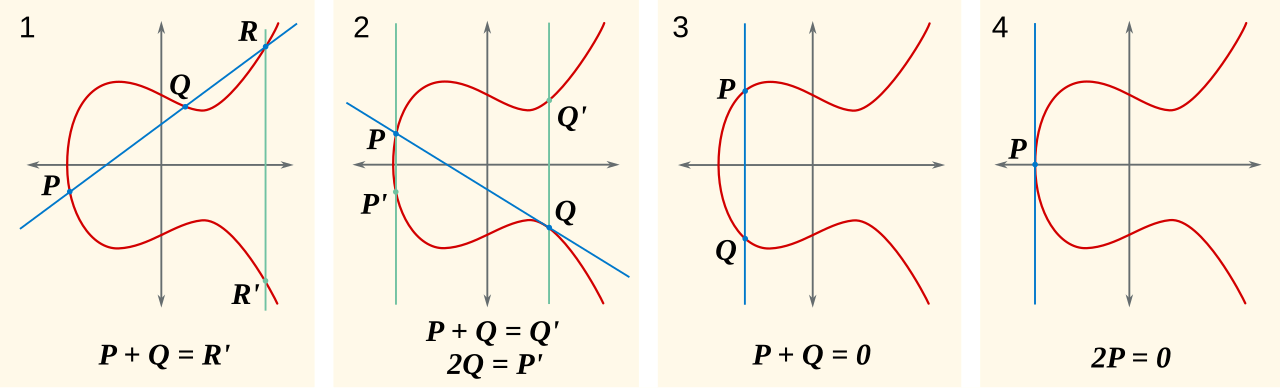
\includegraphics[width=15cm]{EC_add.png}
  \hfuzz=10pt
  \vspace{0cm}
  \caption{Différents cas d'addition dans les courbes elliptiques\cite{frwiki:218649671}}
  \label{fig:addition}
\end{figure}



%-------- Bibliography --------
\newpage
\section{Bibliographie}

\printbibliography

\end{document}

